% ### Erste Seite des Impulssatzes ###
\centering
\vspace{44mm}
\section*{\myul{Impulssatz}}

\begin{tikzpicture}[remember picture, overlay]

% --- ERSTE REIHE: Am Seitenursprung anfangen
\setlength{\rowheight}{44mm}

    % X1) Eigene Zeile für die Überschrift
    \setlength{\cellwidth}{190mm}
    \Tile{X1}{([xshift=10mm, yshift=-81mm]current page.north west)}{\cellwidth}{6mm}
        {
            \vspace{-\TileSep}
            \titlebf{Differentialform}
        }{0}{0}{0}{0}

    % A1) Erste Kachel unten anbauen
    \setlength{\cellwidth}{110mm}
    \Tile{A1}{(X1.south west)}{\cellwidth}{\rowheight}
        {
            \vspace{-\TileSep}
            \titlerm{Konservativ}\\ \vspace{7.5mm}
            \begin{align*}
                \frac{\partial(\rho u)}{\partial t} + \nabla\cdot(\rho\,u\,\underline{v}) &= -\frac{\partial p}{\partial x} + \frac{\partial\tau_{xx}}{\partial x} + \frac{\partial\tau_{yx}}{\partial y} + \frac{\partial\tau_{zx}}{\partial z} + \rho\, f_x \\
                \frac{\partial(\rho v)}{\partial t} + \nabla\cdot(\rho\,u\,\underline{v}) &= -\frac{\partial p}{\partial y} + \frac{\partial\tau_{xy}}{\partial x} + \frac{\partial\tau_{yy}}{\partial y} + \frac{\partial\tau_{zy}}{\partial z} + \rho\, f_y \\
                \frac{\partial(\rho w)}{\partial t} + \nabla\cdot(\rho\,u\,\underline{v}) &= -\frac{\partial p}{\partial x} + \frac{\partial\tau_{xz}}{\partial x} + \frac{\partial\tau_{yz}}{\partial y} + \frac{\partial\tau_{zz}}{\partial z} + \rho\, f_z
            \end{align*}
        }{0}{1}{1}{0}

    % B1) Zweite Kachel rechts anbauen
    \setlength{\cellwidth}{80mm}
    \Tile{B1}{(A1.north east)}{\cellwidth}{\rowheight}
        {
            \vspace{-\TileSep}
            \titlerm{Nicht-Konservativ}\\ \vspace{-3mm}
            \begin{equation*}
                \rho\,\frac{\text{D}\underline{v}}{\text{D}t} = \text{div}\!\left(\underline{\underline{\sigma}}\right) + \rho\,\underline{f}
            \end{equation*}%
            \vspace{-4mm}
            \begin{align*}
                \rho\,\frac{\text{D}(\rho u)}{\text{D} t} &= -\frac{\partial p}{\partial x} + \frac{\partial\tau_{xx}}{\partial x} + \frac{\partial\tau_{yx}}{\partial y} + \frac{\partial\tau_{zx}}{\partial z} + \rho\, f_x \\
                \rho\,\frac{\text{D}(\rho v)}{\text{D} t} &= -\frac{\partial p}{\partial y} + \frac{\partial\tau_{xy}}{\partial x} + \frac{\partial\tau_{yy}}{\partial y} + \frac{\partial\tau_{zy}}{\partial z} + \rho\, f_y \\
                \rho\,\frac{\text{D}(\rho w)}{\text{D} t} &= -\frac{\partial p}{\partial x} + \frac{\partial\tau_{xz}}{\partial x} + \frac{\partial\tau_{yz}}{\partial y} + \frac{\partial\tau_{zz}}{\partial z} + \rho\, f_z
            \end{align*}
        }{0}{0}{1}{0}

% --- ZWEITE REIHE: Unten anbauen
\setlength{\rowheight}{37mm}

    % A2) Erste Kachel unten anbauen
    \setlength{\cellwidth}{95mm}
    \Tile{A2}{(A1.south west)}{\cellwidth}{\rowheight}
        {
            \titlebf{Integralform}\\ \vspace{-4mm}
            \begin{equation*}
                \iiint_V \frac{\partial\left(\rho\,\underline{v}\right)}{\partial t}\,\text{d}V + \oiint_S \rho\,\underline{v}\left(\underline{v}\cdot\underline{n}\right)\,\text{d}S = \iiint_V \rho\,\underline{f}\,\text{d}V + \oiint_S \underline{\underline{\sigma}}\cdot\underline{\text{d}S}
            \end{equation*}
            \rule{\dimexpr\cellwidth-2\TileSep}{0.5pt} \\ \vspace{0.5mm}
            \titlerm{Stationär}\\ \vspace{-4mm}
            \begin{equation*}
                \frac{\text{d}\underline{I}}{\text{d}t} = \oiint_S \rho\,\underline{v}\left(\underline{v}\cdot\underline{n}\right)\,\text{d}S
            \end{equation*}
        }{0}{1}{1}{0}

    % B2) Zweite Kachel rechts anbauen
    \setlength{\cellwidth}{95mm}
    \Tile{B2}{(A2.north east)}{\cellwidth}{\rowheight}
        {
            \titlebf{Reynold'sches Transporttheorem}\\ \vspace{-1mm}
            \begin{align*}
                \frac{\text{D}B}{\text{D}t} &= \frac{\text{D}}{\text{D}t}\,\iiint_{V(t)} b(t)\,\text{d}V = \iiint_{V_0} \frac{\partial b}{\partial t}\,\text{d}V + \iiint_{V_0} \text{div}\!\left(b\,\underline{v}\right)\,\text{d}V \\[2.0ex]
                \frac{\text{D}\underline{B}}{\text{D}t} &= \frac{\text{D}}{\text{D}t}\,\iiint_{V(t)} \underline{b}(t)\,\text{d}V = \iiint_{V_0} \frac{\partial\underline{b}}{\partial t}\,\text{d}V + \oiint_S \underline{b}\left(\underline{v}\cdot\underline{n}\right)\,\text{d}S
            \end{align*}
        }{0}{0}{1}{0}

% --- DRITTE REIHE: Unten anbauen
\setlength{\rowheight}{80mm}

    % A3) Erste Kachel unten anbauen
    \setlength{\cellwidth}{66mm}
    \Tile{A3}{(A2.south west)}{\cellwidth}{\rowheight}
        {
            \titlebf{Praktischer Einsatz}\\ \vspace{3mm}
            \begin{tikzpicture}[node distance=8mm, >=Stealth]
                \node[draw, align=center, rounded corners, minimum width=1cm, minimum height=8mm] (A) {
                    Wahl des Koordinatensystems
                };
                \node[draw, align=center, rounded corners, minimum width=1cm, minimum height=8mm, below=of A] (B) {
                    Wahl des Kontrollvolumens (KV)
                };
                \node[draw, align=center, rounded corners, minimum width=1cm, minimum height=8mm, below=of B] (C) {
                    Zusammenstellung der Kräfte \\
                    $\underline{F} = \underline{F}_p + \underline{F}_f + \underline{F}_\text{K} + \underline{F}_\text{R}$
                };
                \node[draw, align=center, rounded corners, minimum width=1cm, minimum height=8mm, below=of C] (D) {
                    Lösung der Gleichung\\[1.0ex]
                    $\displaystyle\iiint_V \frac{\partial\left(\rho\,\underline{v}\right)}{\partial t}\,\text{d}V + \oiint_S \rho\,\underline{v}\left(\underline{v}\cdot\underline{n}\right)\,\text{d}S = \underline{F} $
                };
                \draw[->] (A) -- (B);
                \draw[->] (B) -- (C);
                \draw[->] (C) -- (D);
            \end{tikzpicture}
        }{0}{1}{1}{0}

    % B3) Zweite Kachel rechts anbauen
    \setlength{\cellwidth}{40mm}
    \Tile{B3}{(A3.north east)}{\cellwidth}{\rowheight}
        {
            \titlebf{Druckkräfte $F_p$}\\ \vspace{-3mm}
            \begin{equation*}
                \text{d}\underline{F}_p = -p\cdot\underline{n}\,\text{d}S
            \end{equation*}
            \begin{equation*}
                \underline{F}_p = -\oiint_S p\,\underline{n}\,\text{d}S
            \end{equation*}%
            \vspace{-1mm}
            \rule{\dimexpr\cellwidth-2\TileSep}{0.5pt} \\ \vspace{0.5mm}
            \titlebf{Volumenkräfte $F_f$}\\ \vspace{-3mm}
            \begin{equation*}
                \underline{F}_\text{f} = \iiint_V \rho\,\underline{f}\,\text{d}V
            \end{equation*}%
            \vspace{1mm}\\
            \titlerm{Schwerefeld}\\ \vspace{-4mm}
            \begin{equation*}
                \text{d}\underline{F}_f = \rho\,\underline{g}\,\text{d}V
            \end{equation*}
            \begin{equation*}
                \underline{F}_f = \iiint_V \rho\,\underline{g}\,\text{d}V
            \end{equation*}
        }{0}{1}{1}{0}

    % C3) Dritte Kachel rechts anbauen
    \setlength{\cellwidth}{84mm}
    \Tile{C3}{(B3.north east)}{\cellwidth}{\rowheight}
        {
            \titlebf{Körperkräfte $F_\mathrm{K}$}\\ \vspace{2mm}
            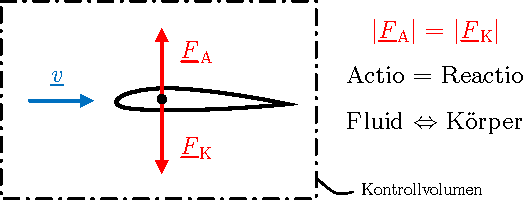
\includegraphics[width=\cellwidth-15mm]{images/körperkräfte.pdf}\\ \vspace{-1mm}
            \rule{\dimexpr\cellwidth-2\TileSep}{0.5pt} \\ \vspace{0.5mm}
            \titlebf{Reibungskräfte $F_\mathrm{R}$}\\ \vspace{2mm}
            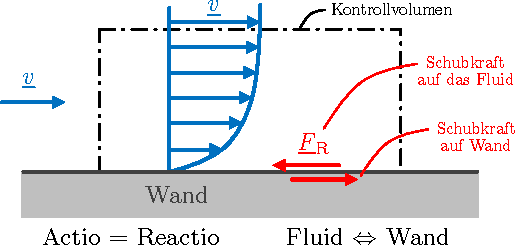
\includegraphics[width=\cellwidth-15.5mm]{images/reibungskräfte.pdf}
        }{0}{0}{1}{0}

% --- VIERTE REIHE: Unten anbauen
\setlength{\rowheight}{24mm}

    % A4) Erste Kachel unten anbauen
    \setlength{\cellwidth}{90mm}
    \Tile{A4}{(A3.south west)}{\cellwidth}{\rowheight}
        {
            \titlebf{Carnot-Diffusor}\\ \vspace{1mm}
            \begin{minipage}[t]{0.5\cellwidth-\TileSep}
                \centering
                \titlerm{Druckdifferenz}\\ \vspace{-4mm}
                \begin{equation*}
                    \Delta p_v = \frac{\rho}{2}\,u_1^2\left(1-\frac{u_2}{u_1}\right)^2
                \end{equation*}
            \end{minipage}%
            \vline
            \begin{minipage}[t]{0.5\cellwidth-\TileSep}
                \centering
                \titlerm{Druckverlustbeiwert}\\ \vspace{-4mm}
                \begin{equation*}
                    \zeta = \frac{2\,\Delta p_v}{\rho\,u_1^2} = \left(1-\frac{A_1}{A_2}\right)^2
                \end{equation*}%
                \vspace{-2mm}
            \end{minipage}
        }{0}{1}{0}{0}

\end{tikzpicture}

% ### Zweite Seite des Impulssatzes ###
\newpage
\centering
\section*{\myul{Impulssatz}}

\begin{tikzpicture}[remember picture, overlay]

% --- ERSTE REIHE: Am Seitenursprung anfangen
\setlength{\rowheight}{45mm}

    % X1) Eigene Zeile für die Überschrift
    \Tile{X1}{([xshift=10mm, yshift=-16mm]current page.north west)}{190mm}{8mm}
        {
            \titlebf{Eulergleichungen}
        }{0}{0}{0}{0}

    % A1) Erste Kachel unten anbauen
    \setlength{\cellwidth}{95mm}
    \Tile{A1}{(X1.south west)}{\cellwidth}{\rowheight}
        {
            \vspace{-\TileSep}
            \titlerm{Konservativ}\\ \vspace{-4mm}
            \begin{equation*}
                \frac{\partial(p\,\underline{v})}{\partial t} + \text{div}\!\left(\rho\cdot\underline{v}\otimes\underline{v}\right) = -\nabla(p) + \rho\,\underline{f}
            \end{equation*}%
            \vspace{-4mm}
            \begin{align*}
                \frac{\partial(\rho\,u)}{\partial t} + \frac{\partial(\rho\,u^2)}{\partial x} + \frac{\partial(\rho\,u\,v)}{\partial y} + \frac{\partial(\rho\,u\,w)}{\partial z} &= -\frac{\partial p}{\partial x} + \rho\,f_x \\[0.5ex]
                \frac{\partial(\rho\,v)}{\partial t} + \frac{\partial(\rho\,v\,u)}{\partial x} + \frac{\partial(\rho\,v^2)}{\partial y} + \frac{\partial(\rho\,v\,w)}{\partial z} &= -\frac{\partial p}{\partial y} + \rho\,f_y \\[0.5ex]
                \frac{\partial(\rho\,w)}{\partial t} + \frac{\partial(\rho\,w\,u)}{\partial x} + \frac{\partial(\rho\,w\,v)}{\partial y} + \frac{\partial(\rho\,w^2)}{\partial z} &= -\frac{\partial p}{\partial z} + \rho\,f_z
            \end{align*}
        }{0}{1}{1}{0}

    % B1) Zweite Kachel rechts anbauen
    \setlength{\cellwidth}{95mm}
    \Tile{B1}{(A1.north east)}{\cellwidth}{\rowheight}
        {
            \vspace{-\TileSep}
            \titlerm{Nicht-Konservativ}\\ \vspace{-3.75mm}
            \begin{equation*}
                \rho\,\frac{\text{D}\underline{v}}{\text{D} t} = \rho\left[\frac{\partial\underline{v}}{\partial t} + \underline{v}\cdot\nabla(\underline{v})\right] = -\nabla(p) + \rho\,\underline{f}
            \end{equation*}%
            \vspace{-3.5mm}
            \begin{align*}
                \rho\,\frac{\partial u}{\partial t} + \rho\,u\,\frac{\partial u}{\partial x} + \rho\,v\,\frac{\partial u}{\partial y} + \rho\,w\,\frac{\partial u}{\partial z} &= -\frac{\partial p}{\partial x} + \rho\,f_x \\[0.5ex]
                \rho\,\frac{\partial v}{\partial t} + \rho\,u\,\frac{\partial v}{\partial x} + \rho\,v\,\frac{\partial v}{\partial y} + \rho\,w\,\frac{\partial v}{\partial z} &= -\frac{\partial p}{\partial x} + \rho\,f_x \\[0.5ex]
                \rho\,\frac{\partial w}{\partial t} + \rho\,u\,\frac{\partial w}{\partial x} + \rho\,v\,\frac{\partial w}{\partial y} + \rho\,w\,\frac{\partial w}{\partial z} &= -\frac{\partial p}{\partial x} + \rho\,f_x
            \end{align*}
        }{0}{0}{1}{0}

% --- ZWEITE REIHE: Unten anbauen
\setlength{\rowheight}{17mm}

    % X2) Eigene Zeile für die Überschrift
    \Tile{X2}{(A1.south west)}{190mm}{14mm}
        {
            \titlebf{Bernoulligleichungen}\\ \vspace{2mm}
            \titlerm{{\color{PineGreen}Stationär}, {\color{PineGreen}Inkompressibel}, {\color{PineGreen}Reibungsfrei}}
        }{0}{0}{0}{0}

    % A2) Erste Kachel unten anbauen
    \setlength{\cellwidth}{48mm}
    \Tile{A2}{(X2.south west)}{\cellwidth}{\rowheight}
        {
            \vspace{-\TileSep}
            \titlerm{Allgemein}\\ \vspace{-4mm}
            \begin{equation*}
                \rho_0\,\frac{v^2}{2} + p + \rho_0\,U = \text{konst.}
            \end{equation*}
        }{0}{1}{1}{0}

    % B2) Zweite Kachel rechts anbauen
    \setlength{\cellwidth}{48mm}
    \Tile{B2}{(A2.north east)}{\cellwidth}{\rowheight}
        {
            \vspace{-\TileSep}
            \titlerm{Energieform}\\ \vspace{-4mm}
            \begin{equation*}
                \frac{v^2}{2} + \frac{p}{\rho} + g\,z = \text{konst.}
            \end{equation*}
        }{0}{1}{1}{0}

    % C2) Zweite Kachel rechts anbauen
    \setlength{\cellwidth}{47mm}
    \Tile{C2}{(B2.north east)}{\cellwidth}{\rowheight}
        {
            \vspace{-\TileSep}
            \titlerm{Druckform}\\ \vspace{-2.75mm}
            \begin{equation*}
                \frac{\rho}{2}\,v^2 + p + \rho\,g\,z = \text{konst.}
            \end{equation*}
        }{0}{1}{1}{0}

    % D2) Zweite Kachel rechts anbauen
    \setlength{\cellwidth}{47mm}
    \Tile{D2}{(C2.north east)}{\cellwidth}{\rowheight}
        {
            \vspace{-\TileSep}
            \titlerm{Höhenform}\\ \vspace{-4mm}
            \begin{equation*}
                \frac{v^2}{2\,g} + \frac{p}{\rho\,g} + z = \text{konst.}
            \end{equation*}
        }{0}{0}{1}{0}

% --- DRITTE REIHE: Unten anbauen
\setlength{\rowheight}{25mm}

    % A3) Erste Kachel unten anbauen
    \setlength{\cellwidth}{123mm}
    \Tile{A3}{(A2.south west)}{\cellwidth}{\rowheight}
        {
            \titlerm{{\color{Mulberry}Instationär}, {\color{PineGreen}Inkompressibel}, {\color{PineGreen}Reibungsfrei}}\\ \vspace{1mm}
            \begin{minipage}[t]{0.61\cellwidth-\TileSep}
                \centering
                \titlerm{Allgemein}\\ \vspace{-3mm}
                \begin{equation*}
                    \int_1^2 \frac{\partial v}{\partial t}\,\text{d}s + \frac{v_2^2 - v_1^2}{2} + \frac{p_2 - p_1}{\rho} + g\left(z_2 - z_1\right) = 0
                \end{equation*}
            \end{minipage}%
            \vrule
            \begin{minipage}[t]{0.39\cellwidth-\TileSep}
                \centering
                \titlerm{Querdruckgleichung}\\ \vspace{-3mm}
                \begin{equation*}
                    \frac{\partial v_n}{\partial t} - \frac{v^2}{r} + \frac{1}{\rho}\,\frac{\partial p}{\partial n} + g\,\frac{\partial z}{\partial n} = 0
                \end{equation*}%
                \vspace{-2mm}
            \end{minipage}
        }{0}{1}{1}{0}

    % B3) Zweite Kachel rechts anbauen
    \setlength{\cellwidth}{67mm}
    \Tile{B3}{(A3.north east)}{\cellwidth}{\rowheight}
        {
            \titlerm{{\color{Mulberry}Instationär}, {\color{Mulberry}Kompressibel}, {\color{PineGreen}Reibungsfrei}}\\ \vspace{1mm}
            \titlerm{Allgemein}\\ \vspace{-3mm}
            \begin{equation*}
                \int_1^2 \frac{\partial v}{\partial t}\,\text{d}s + \frac{v_2^2 - v_1^2}{2} + \int_1^2 \frac{\text{d}p}{\rho} + U_2 - U_1 = 0
            \end{equation*}
        }{0}{0}{1}{0}

% --- VIERTE REIHE: Unten anbauen
\setlength{\rowheight}{25mm}

    % X4) Eigene Zeile für die Überschrift
    \Tile{X4}{(A3.south west)}{190mm}{8mm}
        {
            \titlebf{Anwendungen}
        }{0}{0}{0}{0}

    % A4) Erste Kachel unten anbauen
    \setlength{\cellwidth}{95mm}
    \Tile{A4}{(X4.south west)}{\cellwidth}{\rowheight}
        {
            \titlebf{Venturi-Rohr}\\ \vspace{1mm}
            \begin{minipage}[t]{0.5\cellwidth-\TileSep}
                \centering
                \titlerm{Druckdifferenz}\\ \vspace{-4.5mm}
                \begin{equation*}
                    \Delta p = \frac{\rho}{2}\,v_1^2\left[1 - \left(\frac{A_1}{A_2}\right)^2\right]
                \end{equation*}
            \end{minipage}%
            \vrule
            \begin{minipage}[t]{0.5\cellwidth-\TileSep}
                \centering
                \titlerm{Massenstrom}\\ \vspace{-4.5mm}
                \begin{equation*}
                    \dot{m} = A_1\,A_2\,\sqrt{\frac{2\,\rho\,\Delta p}{A_2^2 - A_1^2}}
                \end{equation*}%
                \vspace{-1.5mm}
            \end{minipage}
        }{0}{1}{1}{0}

    % B4) Zweite Kachel rechts anbauen
    \setlength{\cellwidth}{95mm}
    \Tile{B4}{(A4.north east)}{\cellwidth}{\rowheight}
        {
            \titlebf{Ausströmen aus Gefäß}\\ \vspace{1mm}
            \begin{minipage}[t]{0.5\cellwidth-\TileSep}
                \centering
                \titlerm{Konstanter Spiegel}\\ \vspace{-4.5mm}
                \begin{equation*}
                    v_2 = \sqrt{\frac{2}{\rho}\left(p_1 - p_2\right) + 2\,g\,h}
                \end{equation*}
            \end{minipage}%
            \vrule
            \begin{minipage}[t]{0.5\cellwidth-\TileSep}
                \centering
                \titlerm{Mit Spiegelabsenkung}\\ \vspace{-4.5mm}
                \begin{equation*}
                    \Delta t = \frac{A_1}{A_2}\,\sqrt{\frac{2}{g}}\left(\sqrt{z_1}-\sqrt{z_2}\right)
                \end{equation*}%
                \vspace{-1.5mm}
            \end{minipage}
        }{0}{0}{1}{0}

% --- FÜNFTE REIHE: Unten anbauen
\setlength{\rowheight}{60mm}

    % A5) Erste Kachel unten anbauen
    \setlength{\cellwidth}{115mm}
    \Tile{A5}{(A4.south west)}{\cellwidth}{\rowheight}
        {
            \titlebf{Prandtl-Rohr}\\ \vspace{1mm}
            \titlerm{Inkompressibel}\\ \vspace{1mm}
            \begin{minipage}[t]{0.5\cellwidth-\TileSep}
                \centering
                \titlerm{Druckdifferenz}\\ \vspace{-2.5mm}
                \begin{equation*}
                    \Delta p = p_0 - p_\infty = \rho_\text{F}\,g\,\Delta z
                \end{equation*}
            \end{minipage}%
            \vrule
            \begin{minipage}[t]{0.5\cellwidth-\TileSep}
                \centering
                \titlerm{Anströmgeschwindigkeit}\\ \vspace{-4.5mm}
                \begin{equation*}
                    v_\infty = \sqrt{\frac{2\,\Delta p}{\rho}} = \sqrt{2\,\frac{\rho_\text{F}}{\rho}\,g\,\Delta z}
                \end{equation*}%
                \vspace{-1mm}
            \end{minipage}%
            \vspace{1.75mm}
            \rule{\dimexpr\cellwidth-2\TileSep}{0.5pt} \\ \vspace{0.5mm}
            \titlerm{Kompressibel}\\ \vspace{1mm}
            \begin{minipage}[t]{0.45\cellwidth-\TileSep}
                \centering
                \titlerm{Fehlerabschätzung}\\ \vspace{-4.5mm}
                \begin{equation*}
                    \frac{v_{\infty\text{,\,komp.}}}{v_{\infty\text{,\,inkomp.}}} \approx \sqrt{1 - \frac{\mathrm{Ma}^2_\infty}{4}}
                \end{equation*}
            \end{minipage}%
            \vrule
            \begin{minipage}[t]{0.55\cellwidth-\TileSep}
                \centering
                \titlerm{Anströmgeschwindigkeit}\\ \vspace{-4.5mm}
                \begin{equation*}
                    v_\infty = \sqrt{\frac{2\,\kappa}{\kappa - 1}\,\frac{p_\infty}{\rho_\infty}\left[\left(\frac{p_0}{p_\infty}\right)^{\frac{\kappa-1}{\kappa}}-1\right]}
                \end{equation*}%
                \vspace{-1mm}
            \end{minipage}
        }{0}{1}{1}{0}

    % B5) Zweite Kachel rechts anbauen
    \setlength{\cellwidth}{75mm}
    \Tile{B5}{(A5.north east)}{\cellwidth}{\rowheight}
        {
            \titlebf{Schwingende Säule}\\ \vspace{-3mm}
            \begin{equation*}
                x = x_0\,\cos\!\left(\omega\,t\right)
            \end{equation*}
            \rule{\dimexpr\cellwidth-2\TileSep}{0.5pt} \\ \vspace{0.5mm}
            \titlebf{Bewegung auf konzentrischen Bahnen}\\ \vspace{-3mm}
            \begin{equation*}
                p(r) = p_1 + \frac{\rho}{2}\,v_1^2\left(1-\frac{r_1^2}{r_2^2}\right)
            \end{equation*}
        }{0}{0}{1}{0}

% --- SECHSTE REIHE: Unten anbauen
\setlength{\rowheight}{100mm}

    % A6) Erste Kachel unten anbauen
    \setlength{\cellwidth}{190mm}
    \Tile{A6}{(A5.south west)}{\cellwidth}{\rowheight}
        {
            \vspace{2mm}
            \begin{tabular}{l|c|c|c|c}
                \xrowht[()]{5mm}                   & \cellcolor{Gray!40}Symbol          & \cellcolor{Gray!40}Inkompressibel & \cellcolor{Gray!40}Kompressibel $\left(\mathrm{Ma} \leq 1\right)$ & \cellcolor{Gray!40}Kompressibel $\left(\mathrm{Ma} > 1\right)$ \\ \hline
                \xrowht[()]{5mm} \cellcolor{Gray!40}Statischer Druck  & $p$, $p_\text{s}$, $p_\text{stat}$  & $p$                             & $p$                                            & $p$                                         \\ \hline
                \xrowht[()]{5mm} \cellcolor{Gray!40}Staudruck         & $q$, $p_\text{dyn}$                 & $p_\text{dyn} = p_0 - p = \frac{\rho}{2}\,v^2$ & $p_\text{dyn} = p_0 - p > \frac{\rho}{2}\,v^2$                & \\ \hline
                \xrowht[()]{5mm} \cellcolor{Gray!40}Totaldruck & $p_0$, $p_\text{t}$, $p_\text{ges}$ & $p_0 = p + \frac{\rho}{2}\,v^2$ & \multicolumn{2}{c}{$p_0 = p + \frac{\rho}{2}\,v^2 + \Delta p_\text{komp.} = p\left(1 + \frac{\kappa-1}{2}\,\mathrm{Ma}^2\right)^{\frac{\kappa-1}{\kappa}}$} \\ \hline
                \xrowht[()]{5mm} \cellcolor{Gray!40}Pitotdruck        & $p_\text{pitot}$                    & $p_\text{pitot} = p_0$          & $p_\text{pitot} = p_0$                         & $p_\text{pitot} \leq p_0$
            \end{tabular}
        }{0}{0}{0}{0}

\end{tikzpicture}